\documentclass[12pt,a4paper]{article}
\usepackage[utf8]{inputenc}
\usepackage[T1]{fontenc}
\usepackage{amsmath}
\usepackage{amsfonts}
\usepackage{amssymb}
\usepackage{graphicx}
\usepackage[left=2.54cm, right=2.54cm, top=2.54cm, bottom=2.54cm]{geometry}
\usepackage[hidelinks]{hyperref} %for reference automatically
\usepackage{fancyhdr}

\pagestyle{fancy} % for header and footer
\fancyhf{}
\fancyhead[LE,RO]{Prepared by: Phayuth}
\fancyhead[RE,LO]{Supervisor : Dr.Sarot Srang}
\fancyfoot[LE,RO]{Page \thepage}
\renewcommand{\headrulewidth}{2pt}
\renewcommand{\footrulewidth}{1pt} % for header and footer

% THIS IS THE XML CODE INCLUDE==============================================================
\usepackage{listings}
\usepackage{xcolor}
\definecolor{codegreen}{rgb}{0,0.6,0}
\definecolor{codegray}{rgb}{0.5,0.5,0.5}
\definecolor{codepurple}{rgb}{0.58,0,0.82}
\definecolor{backcolour}{rgb}{0.95,0.95,0.92}
\lstset{
	backgroundcolor=\color{backcolour},   
	commentstyle=\color{codegreen},
	keywordstyle=\color{magenta},
	numberstyle=\tiny\color{codegray},
	stringstyle=\color{codepurple},
	numbers=left,
	breaklines=true,
	tabsize=2,
	basicstyle=\ttfamily\footnotesize,
	literate={\ \ }{{\ }}1
}


\begin{document}
	\section*{\centering Lesson 5 : DC Motor Control}
	\section{Background}
	In application of DC Motor, we want to be able to control its position and angular velocity.
	% \begin{itemize}
	%		\item {\makebox[1cm]{\(\dot{\omega}(t)\)\hfill} is the angular acceleration of dc motor and is the output of the system}
	%		\item {\makebox[1cm]{\(\omega(t)\) \hfill} is the angular velocity of dc motor and is the output of the system}
	%		\item {\makebox[1cm]{\(v_a(t)\)\hfill} is the input voltage to dc motor and is the input of the system}
	%	\end{itemize}
	
	\section{Velocity Control using PI Control (No Nonlinear) (2nd Order Differential Equation Design Workflow)}
	From DC motor Model, we have:
	\begin{equation}
		\label{eq1}
		\dot{\omega}(t) = -a\omega(t) + bv_a(t) 	
	\end{equation}
	We have to design a velocity controller, thus the feedback of the system is angular velocity of the dc motor.\\
	We have our PI control:
	\begin{equation}
		\label{eq2}
		v_a(t) = K_p(\omega_d(t) - \omega(t)) + K_i \int_{0}^{t} (\omega_d(t) - \omega(t)) \,dt
	\end{equation}
	From \autoref{eq1},we get:
	\begin{equation}
		\label{eq3}
		v_a(t) = \frac{1}{b}\dot{\omega}_d(t) + \frac{a}{b}\omega_d(t)
	\end{equation}
	From \autoref{eq2} and \autoref{eq3}, we have our controller design:
	\begin{equation}
		\label{eq4}
		v_a(t) = \frac{1}{b}\dot{\omega}_d(t) + \frac{a}{b}\omega_d(t) + K_p(\omega_d(t) - \omega(t)) + K_i \int_{0}^{t} (\omega_d(t) - \omega(t)) \,dt
	\end{equation}
	\begin{figure}[ht]
		\centering
		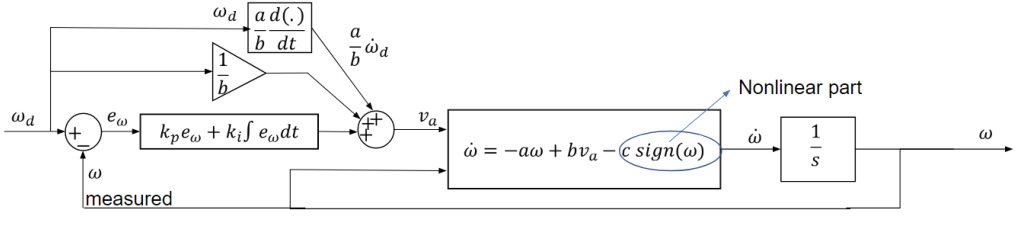
\includegraphics[scale=0.9]{src/img/fig1.pdf}
		\caption{Velocity Control PI Controller}
		\label{fig:Velocity Control PI Controller}
	\end{figure}
	\break
	Substitute \autoref{eq4} back to model in \autoref{eq1}, we get:
	\begin{equation}
		\label{eq5}
		\dot{\omega}(t) = -a\omega(t) + b\left(\frac{1}{b}\dot{\omega}_d(t) + \frac{a}{b}\omega_d(t) + K_p(\omega_d(t) - \omega(t)) + K_i \int_{0}^{t} (\omega_d(t) - \omega(t)) \,dt\right)
	\end{equation}
	\[
	\begin{split}
		0 &= -\dot{\omega}(t) - a\omega(t) + \dot{\omega}_d(t) + a\omega_d(t) + bK_p(\omega_d(t) - \omega(t)) + bK_i \int_{0}^{t} (\omega_d(t) - \omega(t)) \,dt \\
		0 &= (\dot{\omega}_d(t) - \dot{\omega}(t)) + a(\omega_d(t) - \omega(t)) + bK_p(\omega_d(t) - \omega(t)) + bK_i \int_{0}^{t} (\omega_d(t) - \omega(t)) \,dt \\
		0 &= (\dot{\omega}_d(t) - \dot{\omega}(t)) + (a + bK_p)(\omega_d(t) - \omega(t)) + bK_i \int_{0}^{t} (\omega_d(t) - \omega(t)) \,dt \\
		0 &= \dot{e}_{\omega} + (a + bK_p)e_{\omega} + bK_i \int_{0}^{t} e_{\omega}\,dt \\
		0 &= \ddot{e}_{\omega} + (a + bK_p)\dot{e}_{\omega} + bK_ie_{\omega} \leftarrow \text{take derivative to cancel integral.}\\
	\end{split}
	\]
	Thus, we get:
	\begin{equation}
		\label{eq6}
		\ddot{e}_{\omega} + (a + bK_p)\dot{e}_{\omega} + bK_ie_{\omega} = 0
	\end{equation}
	From 2nd Order differential equation standard form, we have:
	\begin{equation}
		\label{eq7}
		\ddot{X} + 2\zeta\omega_nX+\omega_n^2X = 0
	\end{equation}
	From \autoref{eq6} and \autoref{eq7}, we get:
	\[
	\begin{split}
		a + bK_p &= 2\zeta\omega_n \\
		bK_i     &= \omega_n^2 \\
		K_p      &= \frac{2\zeta\omega_n - a}{b} \\
		K_i      &= \frac{\omega_n^2}{b}
	\end{split}
	\]
	From equation above, we want \(K_p > 0\). Thus, \(2\zeta\omega_n > a\), then \(\zeta\omega_n > \frac{a}{2}\) to ensure stability.
	
	
	\section{Velocity Control using PID Control (No Nonlinear) (2nd Order Differential Equation Design Workflow)}
	We have to design a velocity controller, thus the feedback of the system is angular velocity of the dc motor.\\
	We have our PID control:
	\begin{equation}
		\label{eq8}
		v_a(t) = K_p(\omega_d(t) - \omega(t)) + K_i \int_{0}^{t} (\omega_d(t) - \omega(t)) \,dt + K_d \frac{d}{dt} (\omega_d(t) - \omega(t))
	\end{equation}
	From \autoref{eq3} and \autoref{eq8}, we have our controller design:
	\begin{equation}
		\label{eq9}
		v_a(t) = \frac{1}{b}\dot{\omega}_d(t) + \frac{a}{b}\omega_d(t) + K_p(\omega_d(t) - \omega(t)) + K_i \int_{0}^{t} (\omega_d(t) - \omega(t)) \,dt + K_d \frac{d}{dt} (\omega_d(t) - \omega(t))
	\end{equation}
	Substitute \autoref{eq9} back to model in \autoref{eq1}, we get:
	\begin{equation}
		\label{eq10}
		\dot{\omega} = -a\omega + b\left(\frac{1}{b}\dot{\omega}_d + \frac{a}{b}\omega_d + K_p(\omega_d - \omega) + K_i \int_{0}^{t} (\omega_d - \omega) \,dt + K_d \frac{d}{dt} (\omega_d - \omega) \right)
	\end{equation}
	\[
	\begin{split}
		0 &= -\dot{\omega} -a\omega + b(\frac{1}{b}\dot{\omega}_d + \frac{a}{b}\omega_d + K_p(\omega_d - \omega) + K_i \int_{0}^{t} (\omega_d - \omega) \,dt + K_d \frac{d}{dt} (\omega_d - \omega)) \\
		0 &= -\dot{\omega} -a\omega + \dot{\omega}_d + a\omega_d + bK_p(\omega_d - \omega) + bK_i \int_{0}^{t} (\omega_d - \omega) \,dt + bK_d \frac{d}{dt} (\omega_d - \omega) \\
		0 &= (\dot{\omega}_d -\dot{\omega}) + (a+bK_p)(\omega_d -\omega) + bK_i \int_{0}^{t} (\omega_d - \omega) \,dt + bK_d \frac{d}{dt} (\omega_d - \omega) \\
		0 &= (1+bK_d)(\dot{\omega}_d -\dot{\omega}) + (a+bK_p)(\omega_d -\omega) + bK_i \int_{0}^{t} (\omega_d - \omega) \,dt \\
		0 &= (1+bK_d)\dot{e}_{\omega} + (a+bK_p)e_{\omega} + bK_i \int_{0}^{t} e_{\omega} \,dt \\
		0 &= (1+bK_d)\ddot{e}_{\omega} + (a+bK_p)\dot{e}_{\omega} + bK_i e_{\omega} \\
	\end{split}
	\]
	Thus, we get:
	\begin{equation}
		\label{eq11}
		\begin{split}
			(1+bK_d)\ddot{e}_{\omega} + (a+bK_p)\dot{e}_{\omega} + bK_ie_{\omega} = 0 \\
			\ddot{e}_{\omega} + \frac{(a+bK_p)}{(1+bK_d)}\dot{e}_{\omega} + \frac{bK_i}{(1+bK_d)} = 0
		\end{split}
	\end{equation}
	From 2nd Order differential equation standard form \autoref{eq7}, we have:
	\[
	\begin{split}
		\frac{(a+bK_p)}{(1+bK_d)} &= 2\zeta\omega_n \\
		\frac{bK_i}{(1+bK_d)}     &= \omega_n^2 \\
	\end{split}
	\]
	We have more freedom to choose Kp Ki Kd.
	
	
	\section{Position Control using PID Control (No Nonlinear) (2/3rd Order Differential Equation Design Workflow)}
	We have to design a position controller, thus the feedback of the system is shaft position of the dc motor.\\
	We have our PID control:
	\begin{equation}
		\label{eq12}
		v_a(t) = K_p(\theta_d(t) - \theta(t)) + K_i \int_{0}^{t} (\theta_d(t) - \theta(t)) \,dt + K_d \frac{d}{dt} (\theta_d(t) - \theta(t))
	\end{equation}
	From \autoref{eq1}, it can be written in form of position as:
	\begin{equation}
		\label{eq13}
		\ddot{\theta}(t) = -a\dot{\theta}(t) + bv_a(t) 
	\end{equation}
	Thus, we get:
	\begin{equation}
		\label{eq14}
		v_a(t) = \frac{1}{b}\ddot{\theta}_d(t) + \frac{a}{b}\dot{\theta}_d(t)
	\end{equation}
	From \autoref{eq13} and \autoref{eq14}, we have our controller design:
	\begin{equation}
		\label{eq15}
		v_a(t) = \frac{1}{b}\ddot{\theta}_d(t) + \frac{a}{b}\dot{\theta}_d(t) + K_p(\theta_d(t) - \theta(t)) + K_i \int_{0}^{t} (\theta_d(t) - \theta(t)) \,dt + K_d \frac{d}{dt} (\theta_d(t) - \theta(t))
	\end{equation}
	Substitute \autoref{eq15} to \autoref{eq13}, we get:
	\begin{equation}
		\label{eq16}
		\ddot{\theta} = -a\dot{\theta} + b\left(\frac{1}{b}\ddot{\theta}_d + \frac{a}{b}\dot{\theta}_d + K_p(\theta_d - \theta) + K_i \int_{0}^{t} (\theta_d - \theta) \,dt + K_d \frac{d}{dt} (\theta_d - \theta)\right)
	\end{equation}
	\[
	\begin{split}
		\ddot{\theta} &= -a\dot{\theta} + \ddot{\theta}_d + a\dot{\theta}_d + bK_p(\theta_d - \theta) + bK_i \int_{0}^{t} (\theta_d - \theta) \,dt + bK_d \frac{d}{dt} (\theta_d - \theta) \\
		0 &= -\ddot{\theta} -a\dot{\theta} + \ddot{\theta}_d + a\dot{\theta}_d + bK_p(\theta_d - \theta) + bK_i \int_{0}^{t} (\theta_d - \theta) \,dt + bK_d \frac{d}{dt} (\theta_d - \theta) \\
		0 &= (\ddot{\theta}_d -\ddot{\theta}) +a(\dot{\theta}_d -\dot{\theta}) + bK_p(\theta_d - \theta) + bK_i \int_{0}^{t} (\theta_d - \theta) \,dt + bK_d (\dot{\theta}_d -\dot{\theta}) \\
		0 &= (\ddot{\theta}_d -\ddot{\theta}) +(a+bK_d)(\dot{\theta}_d -\dot{\theta}) + bK_p(\theta_d - \theta) + bK_i \int_{0}^{t} (\theta_d - \theta) \,dt \\
		0 &= \ddot{e}_{\theta} +(a+bK_d) \dot{e}_{\theta} + bK_pe_{\theta} + bK_i \int_{0}^{t} e_{\theta} \,dt \\
		0 &= \dddot{e}_{\theta} +(a+bK_d) \ddot{e}_{\theta} + bK_p\dot{e}_{\theta} + bK_ie_{\theta} \\
	\end{split}
	\]
	Thus, we get:
	\begin{equation}
		\label{eq17}
		\dddot{e}_{\theta} +(a+bK_d) \ddot{e}_{\theta} + bK_p\dot{e}_{\theta} + bK_ie_{\theta} = 0
	\end{equation}
	is the 3rd order differential equation with the characteristic form of:
	\begin{equation}
		\label{eq18}
		\lambda^3 + (a+bK_d)\lambda^2 + bK_p\lambda + bK_i = 0
	\end{equation}
	From \autoref{eq18}, we know that in 3rd order differential equation characteristic polynomial, there exist 3 roots and at least 1 root is real root (denoted by $\lambda_1$).Thus, we can write:
	\begin{equation}
		\label{eq19}
		\begin{split}
			(\lambda + \lambda_1)(\lambda^2 + 2\zeta\omega_n\lambda + \omega_n^2) &= 0 \\
			\lambda^3 + 2\zeta\omega_n\lambda^2 + \omega_n^2\lambda + \lambda_1\lambda^2 + 2\zeta\omega_n\lambda\lambda_1 + \omega_n^2\lambda_1 &= 0 \\
			\lambda^3 + (2\zeta\omega_n + \lambda_1)\lambda^2 + (2\zeta\omega_n\lambda_1 + \omega_n^2)\lambda + \omega_n^2\lambda_1 &= 0
		\end{split}
	\end{equation}
	From \autoref{eq18} and \autoref{eq19}, we have:
	\[\begin{split}
		a+bK_d &= 2\zeta\omega_n + \lambda_1 \\
		bK_p &= 2\zeta\omega_n\lambda_1 + \omega_n^2 \\
		bK_i &= \omega_n^2\lambda_1 \\
		K_d &= \frac{2\zeta\omega_n + \lambda_1 - a}{b} \\
		K_p &= \frac{2\zeta\omega_n\lambda_1 + \omega_n^2}{b} \\
		K_i &= \frac{\omega_n^2\lambda_1}{b}
	\end{split}\]
\end{document}